\section{Methods and Materials}

\subsection{ANTs volume-based cortical thickness estimation pipeline}

The ANTs cortical thickness estimation workflow is illustrated
in Figure \ref{fig:pipeline}.  The steps are as follows:
\begin{enumerate}
  \item Initial N4 bias correction on input anatomical MRI
  \item Brain extraction using a hybrid segmentation/template-based strategy
  \item Alternation between prior-based segmentation and ``pure tissue''
        posterior probability weighted bias correction using Atropos and N4
  \item DiReCT-based cortical thickness estimation
  \item Optional normalization to specified template and multi-atlas
    cortical parcellation
\end{enumerate}
Each component, including both software and data, is briefly detailed 
below with the relevant references for additional information. 

%We also note that each component is publicly available with all ANTs 
%algorithms available as open source.%
%\footnote{
%http://www.picsl.upenn.edu/ANTS
%}
The coordination of all the algorithmic components is
encapsulated in the shell script {\tt antsCorticalThickness.sh} with
subcomponents delegated to {\tt antsBrainExtraction.sh} 
and {\tt antsAtroposN4.sh}.  A representative script command 
is reproduced in Listing \ref{listing:antsCorticalThickness} for
a single IXI subject to demonstrate the simplicity and
mature status of what we propose in this work and a comparison
with the analogous FreeSurfer command.  
Option descriptions are provided by invoking the
help option, i.e., ``{\tt antsCorticalThickness.sh -h}''.

\lstset{frame = htb,
        framerule = 0.25pt,
        float,
        fontadjust,
        backgroundcolor={\color{listlightgray}},
        basicstyle = {\ttfamily\scriptsize},
        keywordstyle = {\ttfamily\color{listkeyword}\textbf},
        identifierstyle = {\ttfamily},
        commentstyle = {\ttfamily\color{listcomment}\textit},
        stringstyle = {\ttfamily},
        showstringspaces = false,
        showtabs = false,
        numbers = none,
        numbersep = 6pt,
        numberstyle={\ttfamily\color{listnumbers}},
        tabsize = 2,
        language=bash,
        floatplacement=!h,
        caption={\small \baselineskip 12pt Analogous ANTs and FreeSurfer command line calls 
        for a single IXI subject in the evaluation study.
        },
        captionpos=b,
        label=listing:antsCorticalThickness
        }
\begin{lstlisting}
# Processing calls for subject IXI002-Guys-0828-T1

# ANTs
antsCorticalThickness.sh \
  -a IXI/T1/IXI002-Guys-0828-T1.nii.gz \
  -e IXI/template/T_template0.nii.gz \
  -m IXI/template/T_template0ProbabilityMask.nii.gz \
  -f IXI/template/T_template0ExtractionMask.nii.gz \  
  -p IXI/template/Priors/priors%d.nii.gz \
  -o IXI/ANTsResults/IXI002-Guys-0828-

# FreeSurfer  
recon-all \
  -i  IXI/T1/IXI002-Guys-0828-T1.nii.gz \
  -s  IXI002-Guys-0828 \
  -sd IXI/FreeSurferResults/ \
  -all
\end{lstlisting}

\begin{figure*}
  \centering
  \makebox[\textwidth][c]{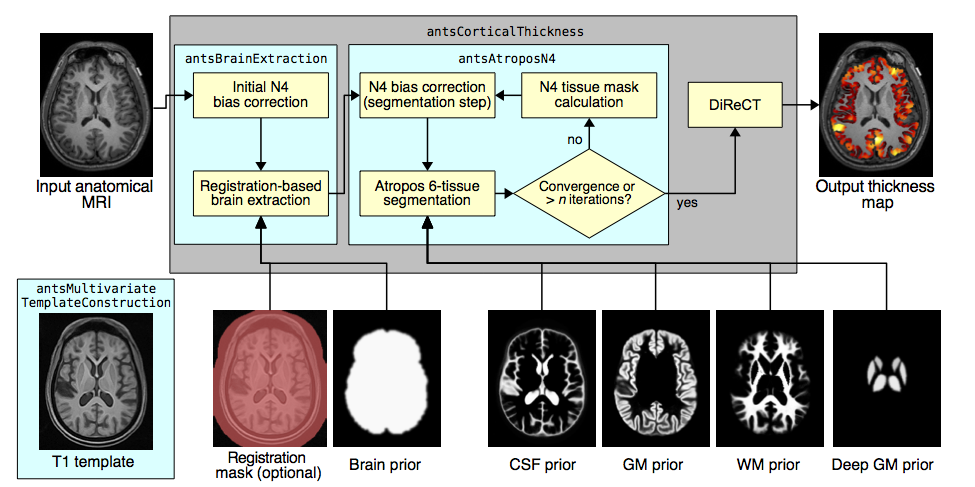
\includegraphics[width=180mm]{Figures/Kapowski_pipeline2.png}}
  \caption{\baselineskip 12pt Illustration of the main components of the ANTs processing 
  workflow containing all elements for determining cortical thickness. 
  We also included the domain of operations for the selected scripts.
  Not shown are the probability maps for the brain stem and cerebellum
  priors.}
  \label{fig:pipeline}
\end{figure*}

\subsubsection{N4 bias field correction}

Critical to quantitative processing of MRI is the minimization of
field inhomogeneity effects which produce artificial low frequency 
intensity variation across the image.  Large-scale studies, such
as ADNI, employ
perhaps the most widely used bias correction algorithm, N3 \citep{sled1998}, 
as part of their standard protocol \citep{boyes2008}.

In \cite{tustison2010} we introduced an improvement of N3, denoted as
``N4'', which demonstrates a significant increase in performance and convergence behavior on a variety of data. 
This improvement is a result of an enhanced
fitting routine (which includes multi-resolution capabilities) and a modified optimization 
formulation.  For our workflow, the additional possibility of specifying
a weighted mask in N4 permits the use of a ``pure tissue'' probability map 
(described below)
calculated during the segmentation pipeline for further improvement of 
bias field estimation.  

N4 is used in two places during the individual subject processing (cf Figure
\ref{fig:pipeline}).  
It is used to generate an initial bias-corrected image for use in
brain extraction.  The input mask is created by adaptively thresholding 
the background from the foreground using Otsu's algorithm \citep{otsu1979}.
Following brain extraction, six-tissue (cerebrospinal fluid, cortical gray 
matter, white matter, deep gray matter, brain stem, and cerebellum)
segmentation involves iterating
between bias field correction using the current pure tissue 
probability map as a weight mask and then using that bias-corrected image
as input for the Atropos segmentation step (described below).

\subsubsection{Brain extraction}

\begin{figure*}
  \vspace{-30mm}
  % 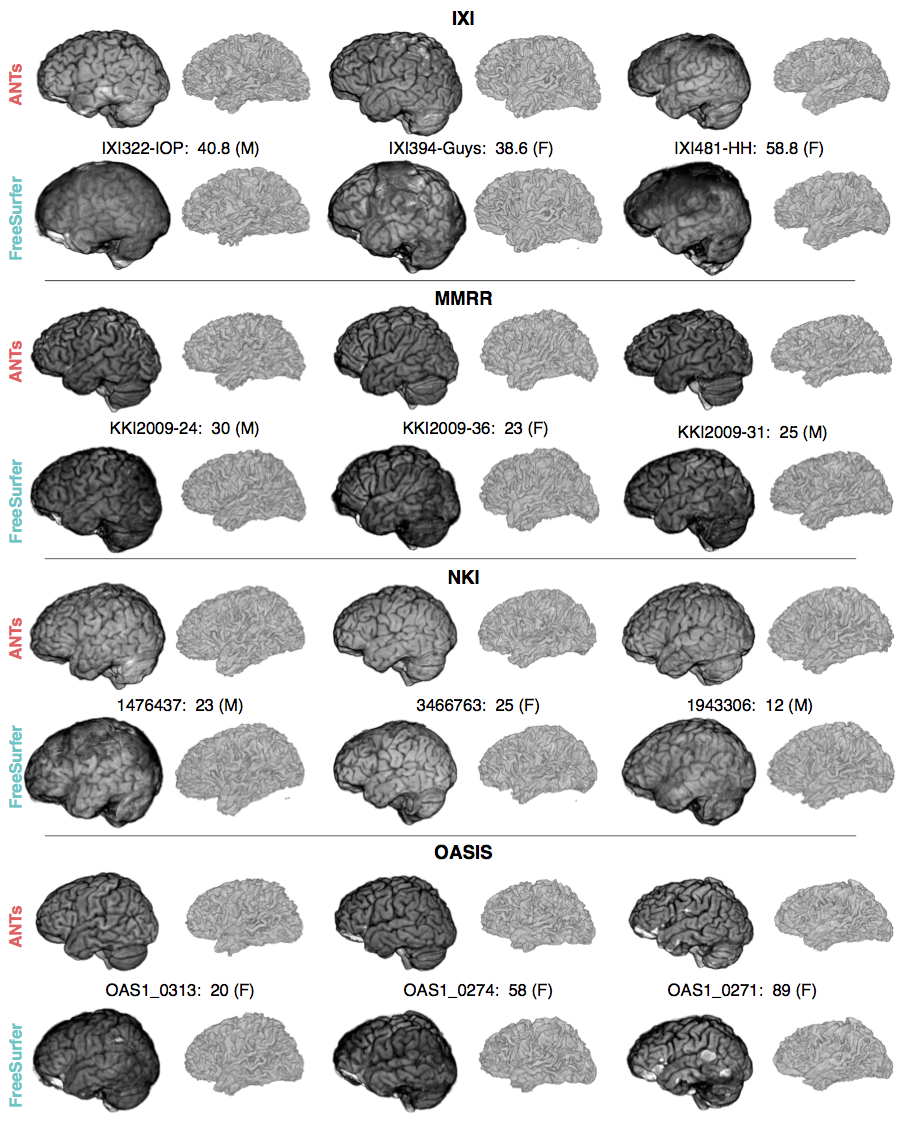
\includegraphics[width=180mm]{montage2.pdf}
  \makebox[\textwidth][c]{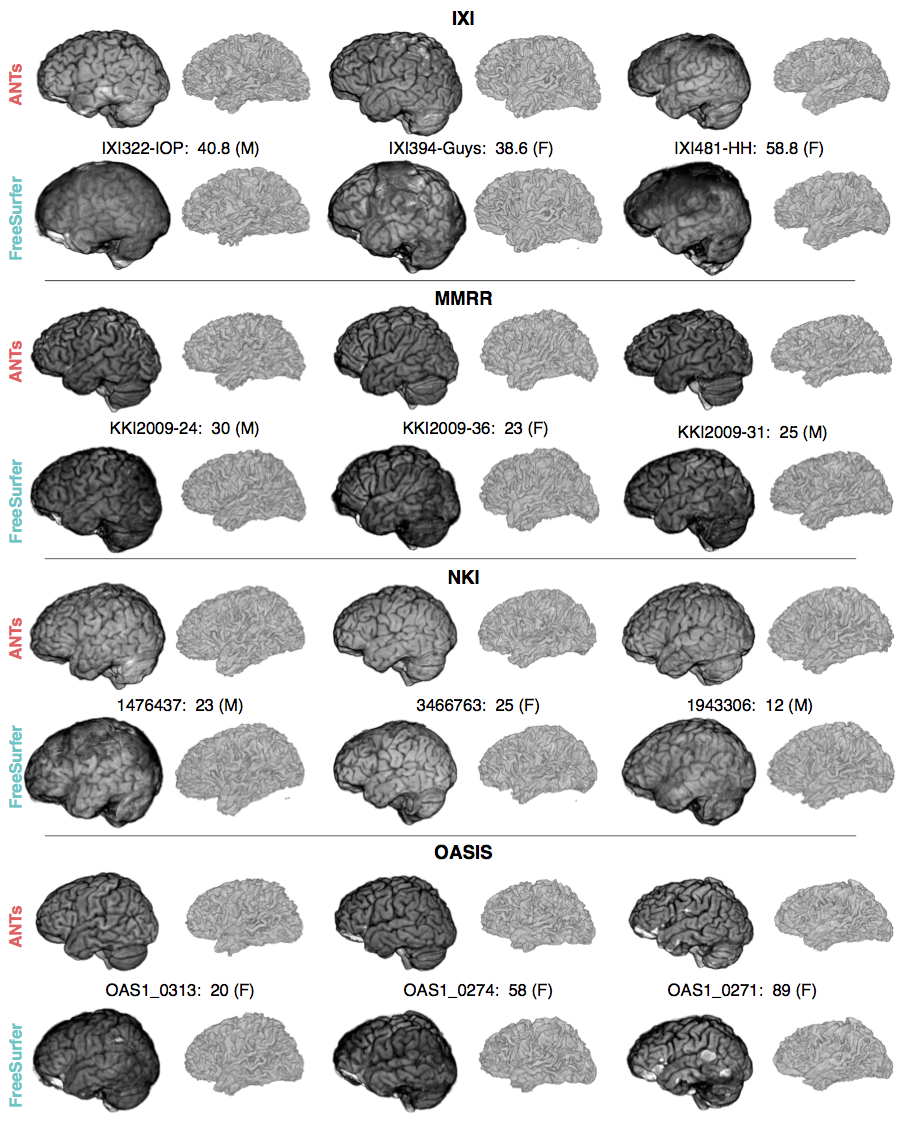
\includegraphics[width=150mm]{montage2.png}}
  \caption{\baselineskip 12pt Representative sample of volume brain renderings from the four
  different cohorts (IXI = rows 1 and 2, MMRR = rows 3 and 4, 
  NKI = rows 5 and 6, OASIS = rows 7 and 8),
  illustrating the qualitative difference between ANTs and FreeSurfer 
  results, which are arranged top-and-bottom for each subject.  Each brain was rigidly
  registered to the OASIS template for rendering purposes.  With each subject
  we provide subject ID, age, and gender.
  }
  \label{fig:brainExtraction}
\end{figure*}

Brain extraction using ANTs combines template building, high-performance
brain image registration, and Atropos segmentation with topological refinements.
An optimal template \citep{avants2010}, i.e., a mean shape and intensity image 
representation of a particular cohort,  is first constructed using structural 
MRI data.  Template construction iterates between estimating
the optimal template and registering each subject to the optimal template.
In this work, we perform the additional step of building separate templates
for each cohort and propagating the probabilistic mask to each cohort template
using registration of the T1-weighted templates (cf Figure \ref{fig:template}).
A probabilistic brain extraction mask for the new template can then be generated 
by warping an existing mask to the template or by averaging the warped, whole brain 
labels of subjects registered to the new template, if such labels are available.
Further refinements include thresholding the warped brain probability map
at 0.5 and dilating the resulting mask with a radius of two.  Atropos is used
to generate an initial three-tissue segmentation estimate within the mask
region.  Each of the three tissue labels undergoes separate morphological  
operations including hole-filling and erosion.  These results are then combined
to create the brain extraction mask which is further refined by additional 
dilation, erosion, and hole-filling operations.  The complete workflow is
found in the script {\tt antsBrainExtraction.sh}.%
\footnote{
A self-contained 2-D example is available at https://github.com/ntustison/antsBrainExtractionExample.
}  

In an evaluation study, we compared an earlier version of our extraction method
with publicly available brain extraction algorithms, including
AFNI's \verb#3dIntracranial#
\citep{ward1999}, FSL's \verb#BET2# \citep{smith2002}, FreeSurfer's
\verb#mri_watershed# \citep{segonne2004}, and BrainSuite
\citep{dogdas2005}. We demonstrated that our combined
registration/segmentation approach \citep{avants2010a} performed
with an accuracy comparable to FreeSurfer and a parameter-tuned version of BrainSuite.
Figure \ref{fig:brainExtraction} presents a visual comparison of results derived with
the current ANTs brain extraction method and results obtained using FreeSurfer.

\subsubsection{Atropos six-tissue segmentation}

In \cite{avants2011a} we presented an open source $n$-tissue segmentation software tool
(which we denote as ``Atropos'') that attempts to distill over 20 years of active research in this area,
in particular some of the most seminal work (e.g., \cite{zhang2001,ashburner2005}).
Specification of prior probabilities includes spatially varying Markov Random Field modeling, 
prior label maps, and prior probability maps typically derived from our template building 
process.  Additional
capabilities include handling of multivariate data, 
partial volume modeling \citep{shattuck2001}, a memory-minimization mode,
label propagation, a plug-and-play architecture for incorporation of novel likelihood models
which includes both parametric and non-parametric models for both scalar and tensorial
images, and alternative posterior formulations for different segmentation tasks.

Due to the important interplay between segmentation and bias correction,
we perform multiple N4 $\rightleftharpoons$ Atropos iterations.
Atropos and N4 are integrated in the script {\tt antsAtroposN4.sh}.%
\footnote{
https://github.com/ntustison/antsAtroposN4Example
}
A pure tissue probability weight mask generated from the 
posterior probabilities is derived from the segmentation 
step.  Given $N$ labels and the corresponding $N$
posterior probability maps $\{ P_1, \ldots, P_N\}$ produced
during segmentation, the N4 weight mask is 
created at each N4 $\rightleftharpoons$ Atropos iteration from
\begin{align}
  P_{pure\,\,tissue}(\mathbf{x}) = \sum_{i=1}^N P_i(\mathbf{x}) \prod_{j=1, j \neq i}^N \left( 1 - P_j(\mathbf{x}) \right).
\end{align}
One of the key insights of the original N3 development is the
observation that inhomogeneities cause the intensity values of
pure tissue peaks to spread in the intensity histogram as though
convolved with a Gaussian.  A core contribution of N3 is the
proposed corrective step of deconvolving the intensity histogram to
accentuate the tissue peaks, coupled with a spatial smoothing
constraint. The pure tissue probability mask is used in N4 to weight
more heavily the influence of voxels corresponding to pure tissue 
types (as determined by the segmentation) during the deconvolution process 
while minimizing the contribution of regions such as the gray/white matter 
interface where peak membership is ambiguous. 

Atropos enables prior knowledge to guide the
segmentation process where template-based priors are integrated into the optimization
with a user-controlled weight.  Modulating the likelihood and prior contributions
to the posterior probability is essential for producing adequate segmentations.
Atropos weights the likelihood and priors according to
$P(x|y) \propto P(y|x)^{1-\alpha}P(x)^{\alpha}$
where $\alpha$ is a user-selected parameter which weights the tradeoff between the likelihood and priors terms.  A weighting of $\alpha = 0.25$ is the default value based 
on our extensive experimentation with different parameter weights.


Since cortical thickness estimation only requires the cortical gray
and white matter, the deep gray and white matter
(both labels and posterior maps) are combined to form a single
``white matter'' set.  This white matter set and the cortical
gray matter are the only results from the segmentation
step that are used by the DiReCT algorithm (described below).


\subsubsection{DiReCT cortical thickness estimation}

DiReCT was introduced 
in \cite{das2009} and was made available in ANTs as the program \verb#KellySlater#.
Since then several improvements have been made and incorporated into the program
\verb#KellyKapowski#.%
\footnote{
Traditional academic discourse encountered in the published literature
rarely contextualizes peculiarities such as algorithmic nomenclature.
We briefly mention that
this was the source of a rare disagreement between the first and last authors
based, as many disagreements are, on a simple misunderstanding and not an
affronting existential statement concerning a certain favorite sitcom
of the first author's youth. 
}
The more recent implementation has made numerous advances, including:
it is multi-threaded, written in rigorous ITK coding style,%
\footnote{
http://www.itk.org/ITK/help/documentation.html
}
 and
has been made publicly available through ANTs, complete with a unique command line
interface design developed specifically for ANTs tools.
Additionally, a fully functional, self-contained example using 2-dimensional image data is 
provided.%
\footnote{
https://github.com/ntustison/antsCorticalThicknessExample
}

\subsubsection{Anatomical template construction}

Normalizing images to a standard coordinate system
reduces intersubject variability in population studies.  Various
approaches exist for determining the standardized coordinate space,
such as the selection of a preexisting template based on a single individual
(e.g., the Talairach atlas \citep{Talairach1988}) or a publicly available average of multiple individuals
(e.g., the MNI \citep{Collins1994} or ICBM \citep{Mazziotta1995}
templates), or an average template constructed from the individuals under study.
The work of \cite{avants2010} explicitly models the geometric component of the 
normalized space during optimization to produce such mean templates.  Coupling the intrinsic symmetry of 
SyN pairwise registration \citep{avants2011} and an
optimized shape-based sharpening/averaging of the template appearance, Symmetric Group Normalization (SyGN) is a powerful framework for producing optimal population-specific templates.

The ANTs implementation of this technique is currently available as a shell script, 
{\tt buildtemplateparallel.sh}.  A generalized, multivariate version is also available as
{\tt antsMultivariateTemplateConstruction.sh}.  Both scripts are distributed as part of
 the ANTs software.  The multivariate script permits the construction of multimodal templates
created from a cohort of subjects, each with a set of pre-aligned multimodal images per subject.  
All modalities are used during the template-building process.  For example, for $N$ subjects where 
each subject has T1, T2, and fractional anisotropy (FA) images which are all aligned in the same subject space, 
a multimodal template consisting 
of T1, T2, and FA components can be created using antsMultivariateTemplateConstruction.sh.
Both scripts accommodate a variety of computational resources
for facilitating template construction.%
\footnote{
A self-contained 2-D example is available at https://github.com/ntustison/TemplateBuildingExample.
}
These computational resource possibilities include:
\begin{itemize}
  \item serial processing on a single workstation
  \item parallelized processing on a single workstation with multiple cores using \verb#pexec#%
  \footnote{http://www.gnu.org/software/pexec/pexec.1.html}
  \item parallelized processing using Apple's XGrid technology%
  \footnote{https://developer.apple.com/hardwaredrivers/hpc/xgrid\_intro.html}
  \item parallelized processing using Sun Grid Engine for cluster-based systems%
  \footnote{http://www.oracle.com/technetwork/oem/grid-engine-166852.html}
  \item parallelized processing using the Portable Batch System for cluster-based systems%
  \footnote{http://www.pbsworks.com/}  
\end{itemize}

For this work, cohort-specific templates were used during cortical thickness pipeline
processing for both brain extraction and segmentation steps.  Further details regarding
the actual templates used (along with corresponding prior probability maps) are given 
in the section describing the public data used.  The quality of prior probability images,
particularly for the segmentation step, is crucial for performance.  

To generate the priors for each T1 template, we used the multi-atlas label fusion (MALF) 
algorithm of \cite{wang2013} which is also distributed with ANTs and simplified with the 
{\tt antsMalfLabeling.sh} script.  We also used the training data associated with the 
MICCAI 2012 Grand Challenge and Workshop on Multi-Atlas Labeling%
\footnote{
https://masi.vuse.vanderbilt.edu/workshop2012/index.php/Main\_Page
}
consisting of 20 labeled brain data taken from the OASIS data set.%
\footnote{
The data was released under the Creative Commons Attribution-NonCommercial license. 
Labelings were provided by Neuromorphometrics, Inc. (http://Neuromorphometrics.com/) 
under academic subscription.
}
Once the labels were propagated to the template, we condensed the 100+ labels associated
with the training data to the six needed for our analysis, viz., cerebrospinal fluid (CSF), 
gray matter (GM), white matter (WM), deep gray matter, brain stem, and cerebellum.  These binary
masks were then smoothed using Gaussian convolution with a one voxel-width kernel (cf
Figure \ref{fig:templateMasks}).  Since the labelings did not describe the extracerebral
CSF, we augmented the CSF prior image with the CSF posterior output from running each template 
through the segmentation component of the above-described pipeline with a template 
that we had built previously.  This new CSF prior was then subtracted from each of the
other five prior probability images.

\subsection{Public data resources}

The above pipeline was run on four publicly available data sets:
IXI, MMRR, NKI, and OASIS. 
In addition, we used a subset of the MindBoggle-101 data%
\footnote{
http://mindboggle.info/data.html
} 
labeled using the 
Desikan-Killiany-Tourville (DKT) protocol \citep{klein2012} to define the
regions of interest (ROI).  This latter data set was not included in the 
thickness analysis.
All five data sets are described below.

\subsubsection{MindBoggle-101 data for ROI definitions}

\begin{table}
\centering
\begin{tabular*}{0.9\textwidth}{@{\extracolsep{\fill}} l l}
\toprule
  1) caudal anterior cingulate & 17) pars orbitalis \\
  2) caudal middle frontal & 18) pars triangularis \\
  3) cuneus &  19) pericalcarine \\
  4) entorhinal & 20) postcentral \\
  5) fusiform &  21) posterior cingulate\\
  6) inferior parietal & 22) precentral \\
  7) inferior temporal & 23) precuneus \\
  8) isthmus cingulate & 24) rosterior anterior cingulate\\
  9) lateral occipital & 25) rostral middle frontal \\
  10) lateral orbitofrontal  & 26) superior frontal \\
  11) lingual & 27) superior parietal \\
  12) medial orbitofrontal & 28) superior temporal \\
  13) middle temporal & 29) supramarginal \\
  14) parahippocampal & 30) transverse temporal \\
  15) paracentral & 31) insula \\
  16) pars opercularis  & {}\\
  \bottomrule
\end{tabular*}
\caption{\baselineskip 12pt The 31 cortical labels (per hemisphere) of the DKT atlas.  }
\label{table:dkt_labels}
\end{table}

In \cite{klein2012} the authors proposed the DKT cortical labeling protocol---a modification of the
popular Desikan-Killiany protocol \citep{desikan2006} to improve cortical labeling
consistency and to improve FreeSurfer's cortical classification of 31 cortical regions per hemisphere,
listed in Table \ref{table:dkt_labels}.
For the latter, forty manually labeled brains were used to construct the DKT40 Gaussian classifier atlas,
which is now bundled with current versions of FreeSurfer and
used to automate anatomical labeling of MRI data.
Since the regional thickness values generated by FreeSurfer follow this protocol,
these anatomical labels provide a common standard for comparison between ANTs and FreeSurfer.

The work of \cite{klein2012} also resulted in a publicly available set of
manually edited labels following the DKT protocol in 101
T1-weighted  brain images from different sources, including a subset of 20 images
from the OASIS data set (specifically, the test-retest data).  
These 20 images are used in the MALF step that defines the volumetric cortical regions 
for each subject.  


\subsubsection{Public data for thickness estimation evaluation}

\begin{figure}
  \centering
%  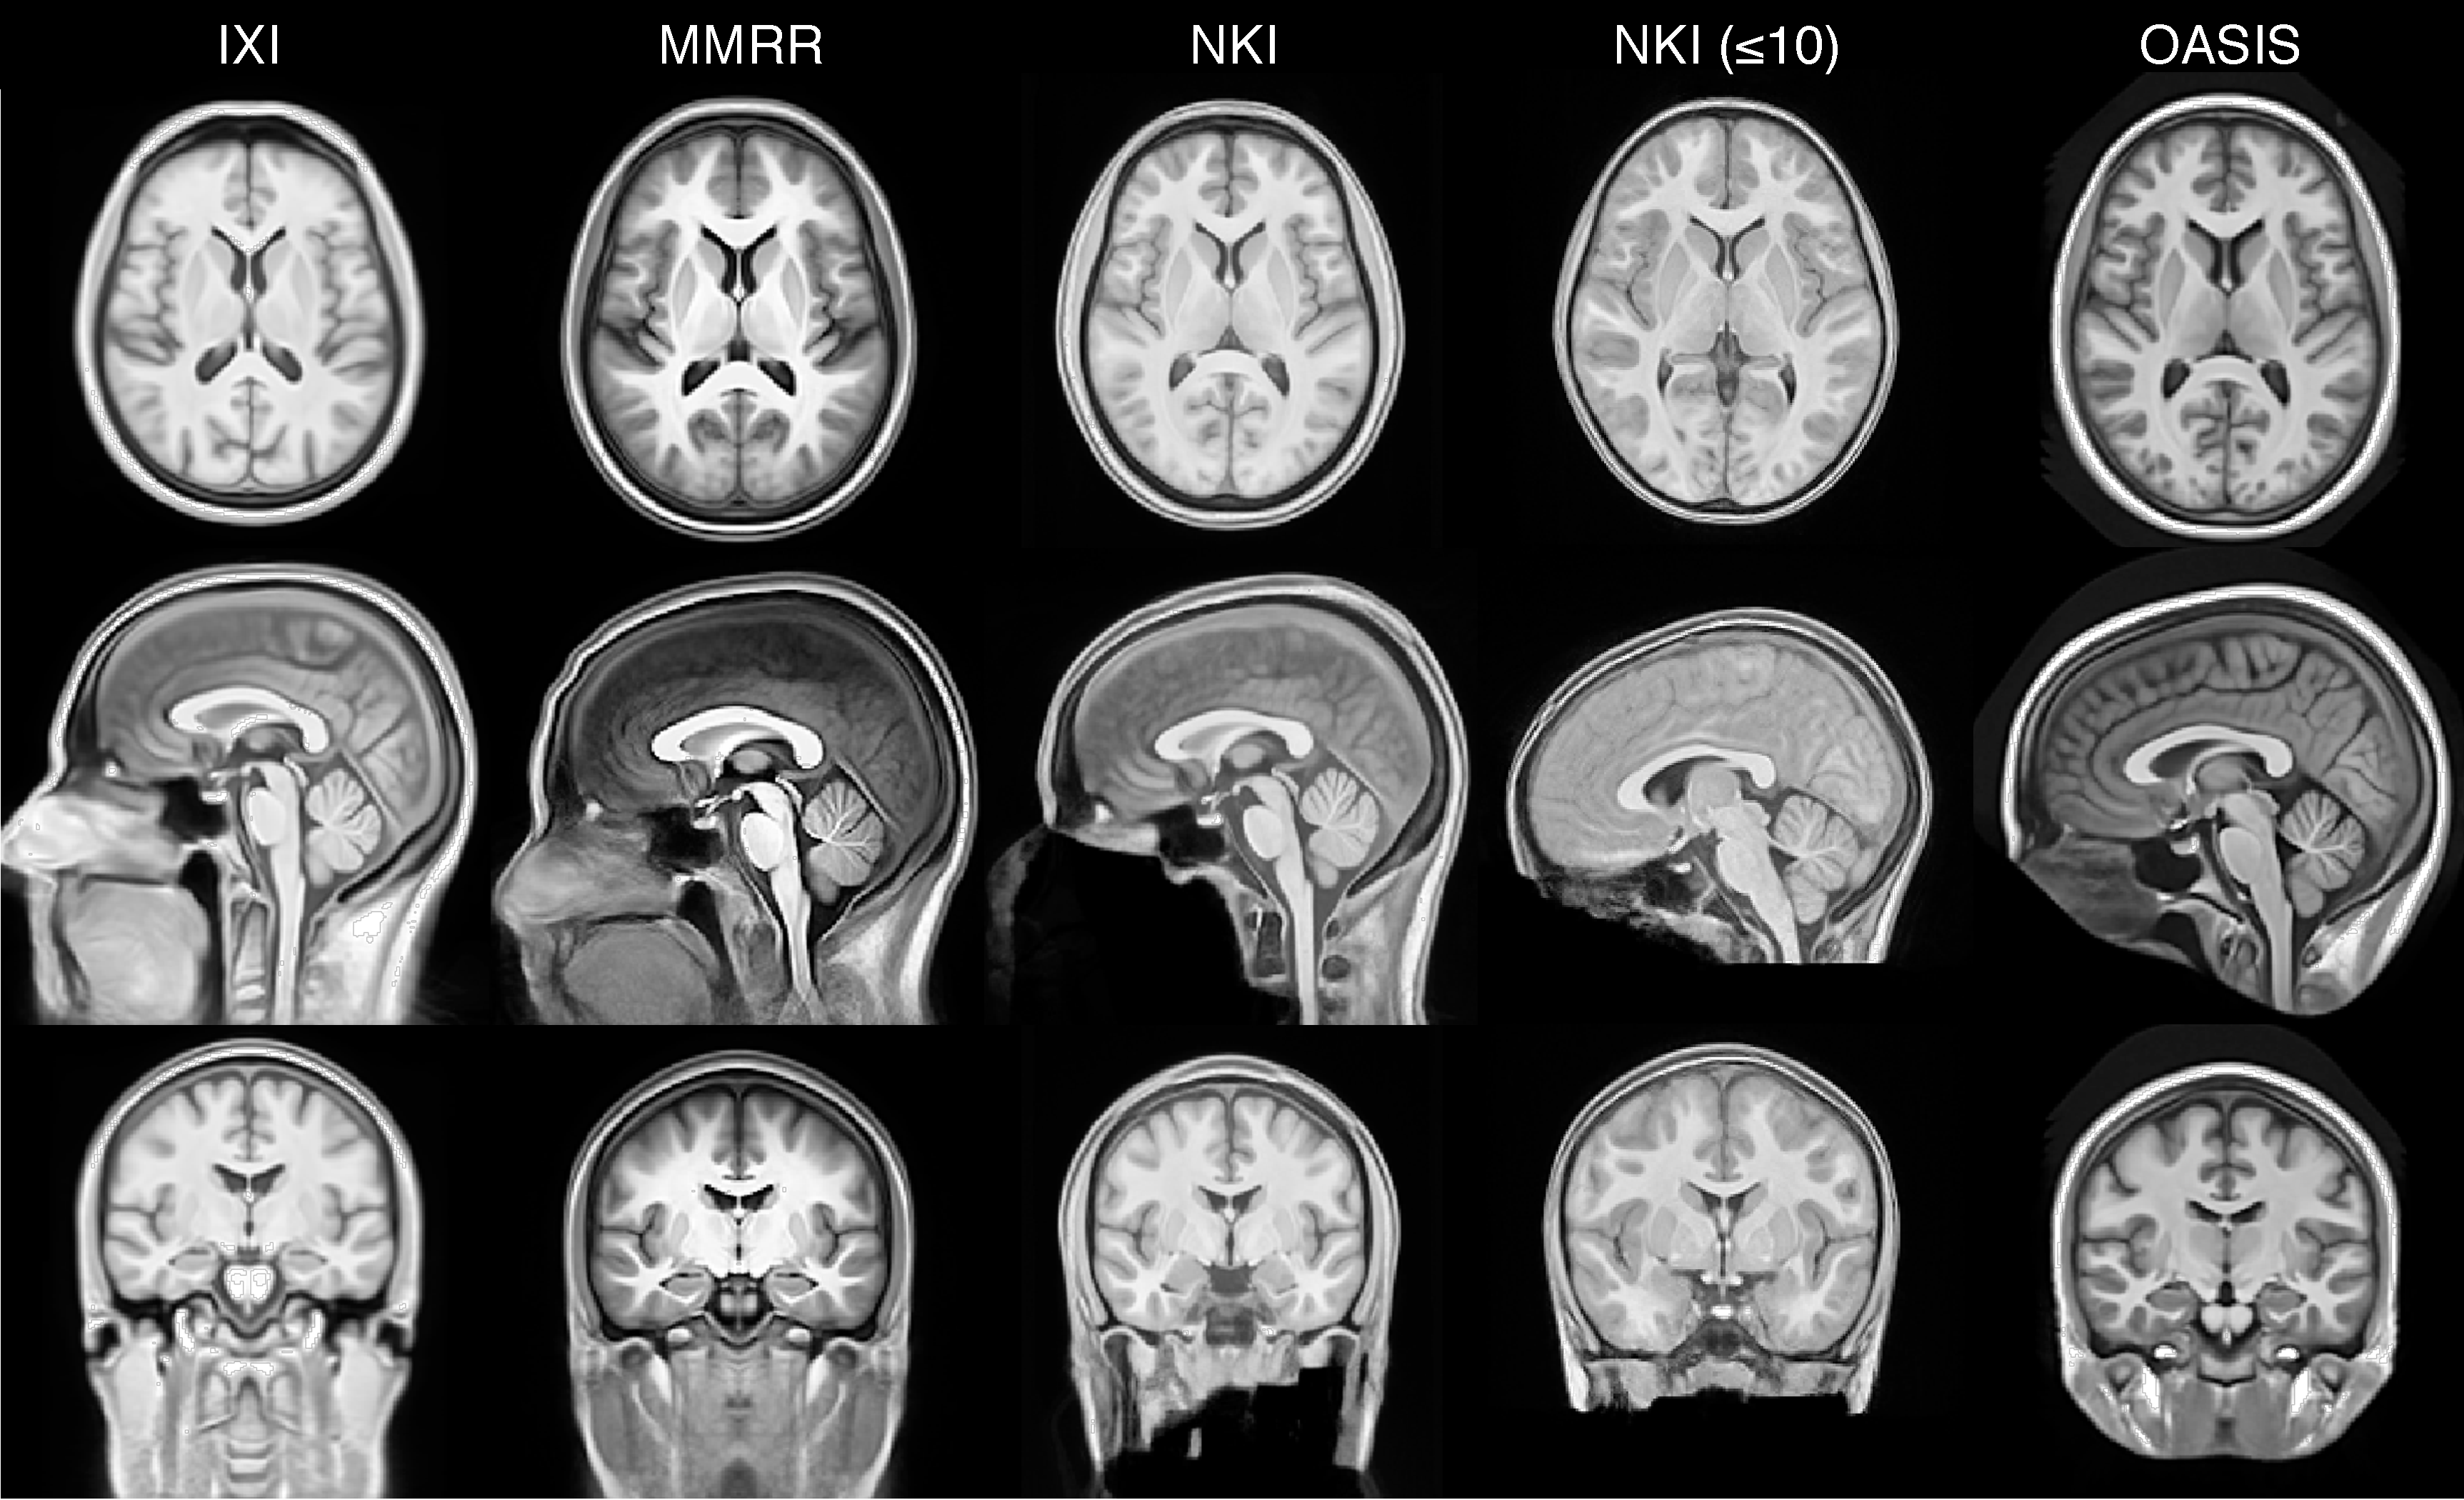
\includegraphics[width=90mm]{Figures/templates.pdf}
  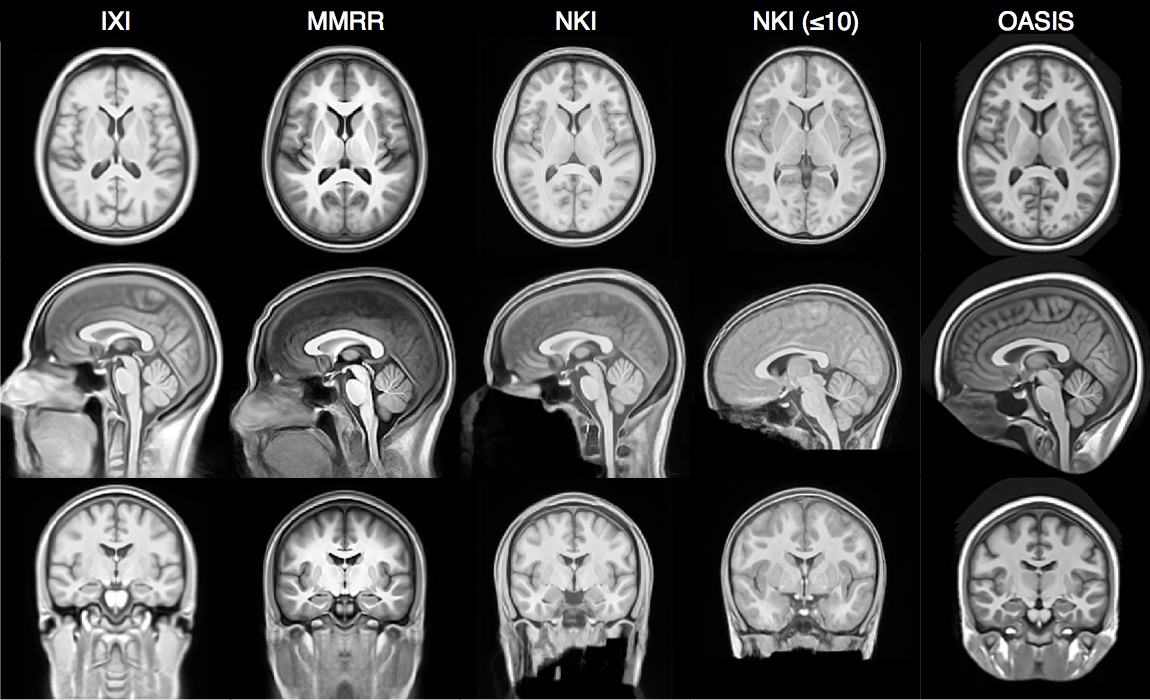
\includegraphics[width=130mm]{Figures/templates.jpg}
  \caption{\baselineskip 12pt Population-specific templates for each of the four public data sets used
  for cortical thickness 
  estimation. These templates were generated using the script {\tt antsMultivariateTemplateConstruction.sh}.
  The benefit of using such population-specific templates is obvious when one sees the variability in
  acquisition and data preparation (e.g., defacing protocols).
  }
  \label{fig:template}
\end{figure}

We applied the same pipeline to diverse publicly available data sets collected
from multiple sites and with a mixture of 3T and
1.5T T1-weighted brain images.  Subjects in this data set  
span the age range from 4 to 96 years old.  This strategy tested robustness to
variation in head position, brain shape, defacing, image contrast, inhomogeneity, imaging
artifacts, field strength, and the broad variation in extracerebral tissue.  Failure
can occur in initial brain extraction, segmentation, registration, or
bias correction, any of which can lead to an inaccurate cortical
thickness measurement.                           

In total, we processed 1,205 T1-weighted images from four different
public data sets to obtain cortical thickness maps.
Below we describe the four data sets and their corresponding
templates%
\footnote
{
Templates and prior probability images are available for download at
http://figshare.com/articles/ANTs\_ANTsR\_Brain\_Templates/915436.
}:
                                          
\paragraph{IXI}
Initially, we processed 581 T1-weighted images from the IXI%
\footnote{
http://biomedic.doc.ic.ac.uk/brain-development/
}
 data set, but only 563 subjects
(313 females, 250 males) were included in the post-processing analysis due to 
missing demographic information, which would have prevented an accurate estimate of
the age at the time of image acquisition.  These data were
imaged at three sites 
with several modalities acquired (T1-weighted, T2-weighted, proton density, magnetic 
resonance angiography, and diffusion tensor imaging).  The 
database also includes demographic information such as date of birth, date
of scan, weight,
height, ethnicity, occupation category, educational level, and marital status.

The IXI template had been built previously during an investigation of  multimodal 
(T1, T2, FA, and proton density) template generation using different 
aged cohorts.  Templates consisting of subjects
within decade ranges, i.e., 10 to 20, 20 to 30, etc. were built.  These
age-based multimodal templates were then used to build an average ``meta-template'' of which 
the T1 component is used in this study as seen, respectively, in the first column and row of 
Figures \ref{fig:template} and \ref{fig:templateMasks}.

\paragraph{MMRR}
The Multi-Modal MRI Reproducibility Resource (MMRR)%
\footnote{
http://www.nitrc.org/projects/multimodal/
} 
data set, was originally described in \cite{landman2011} consisting of 
21 subjects (10 females, 11 males) and features a rich set of modalities, 
as well as repeated scans.

In previously testing our template construction protocol, we used all 
MMRR data sets to construct a multimodal template consisting of
FA, mean diffusivity (MD), FLAIR, T1, T2, magnetic transfer (MT), and 
vascular space occupancy (VASO) components.  More details concerning 
data acquired are provided at \cite{landman2011}.  The T1 component used in 
this study can be seen, respectively, in the second column and row of 
Figures \ref{fig:template} and \ref{fig:templateMasks}.

\paragraph{NKI}
In support of open science, the 1,000 Functional Connectomes Project%
\footnote{ 
http://fcon\_1000.projects.nitrc.org
}
was initiated on December 11, 2009 by various members of the MRI community
seeking to form collaborative partnerships among imaging institutions for
sharing well-documented multimodal image sets accompanied by phenotypic data.
One such contribution is the Nathan Klein Institute (NKI)/Rockland sample,
consisting of 186 T1-weighted
images (87 females, 99 males).%
\footnote{
Downloaded on September 22, 2012.
}

The T1-weighted template was constructed originally for the study performed
in \cite{tustison2013}.  It was created from 30 randomly sampled subjects 
which we repurpose here for our cortical thickness evaluation.  Since the 
NKI cohort contains younger individuals, for this study we also created a 
template for subjects of 10 years and younger generated from 13 individuals.
Both templates and corresponding priors are also seen in Figures \ref{fig:template} and \ref{fig:templateMasks}.

\paragraph{OASIS}
The initial Open Access Series of Imaging Studies (OASIS)%
\footnote{
http://www.OASIS-brains.org/
}
data set consisted of 433 T1-weighted images.  We processed all of these,
but 100 were excluded from our analysis due to probable Alzheimer's
disease ($CDR > 0$) and an additional 20 repeat scans were excluded,
 resulting in 313 individual subject scans included in the normal group statistical
analysis (118 males, 195 females).  Ages were between 18 and 96 and 
all subjects are right-handed.  

As part of the MICCAI 2012 Grand Challenge mentioned earlier, the first and
last authors were asked to provide the ``canonical'' registrations for each
pairwise mapping.  Instead of performing $n^2$ registrations where $n$ is
the number of subjects, we decided to produce all mappings using a 
``pseudo-geodesic'' approach where all subjects are warped to an optimal
template thus providing any pairwise transformation and thereby 
reducing the number of image registrations required from $n^2$ to $n$.
The optimal template for this pseudo-geodesic processing was constructed 
from the combined 35 testing and training OASIS data of the MICCAI 2012 Grand 
Challenge which we repurpose for this study.

\begin{figure}
  \centering
%  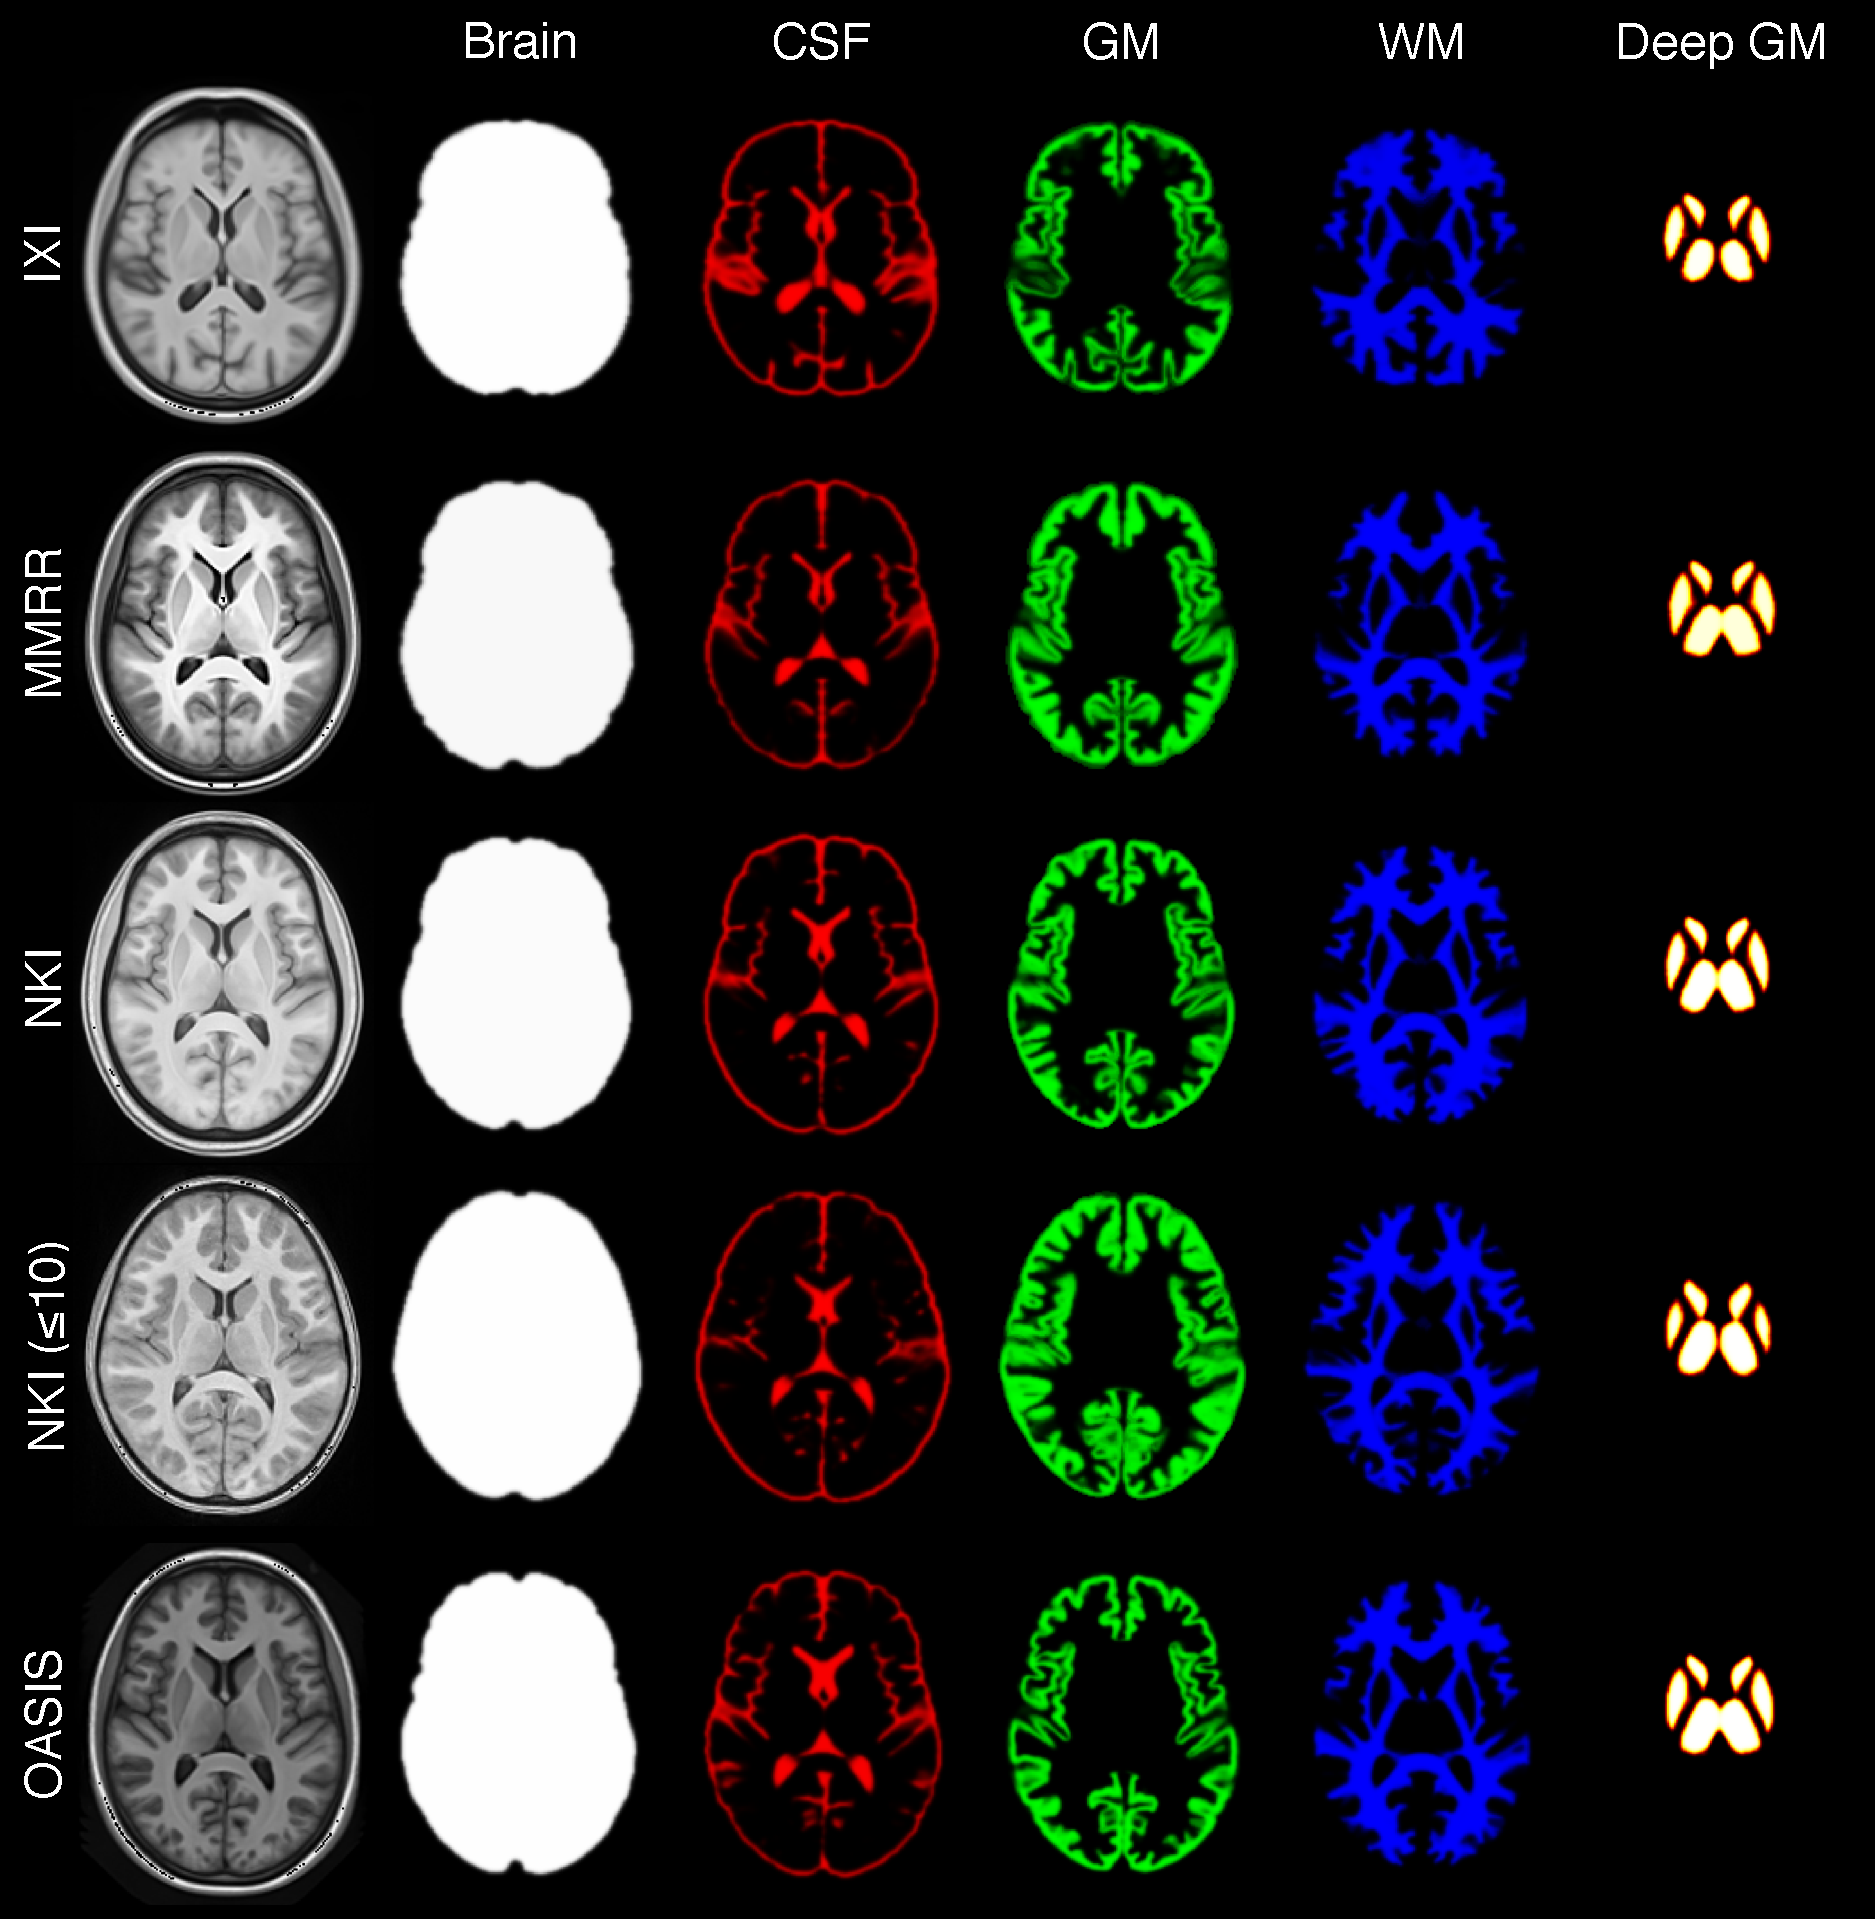
\includegraphics[width=90mm]{Figures/templateProbabilityMasks.pdf}
  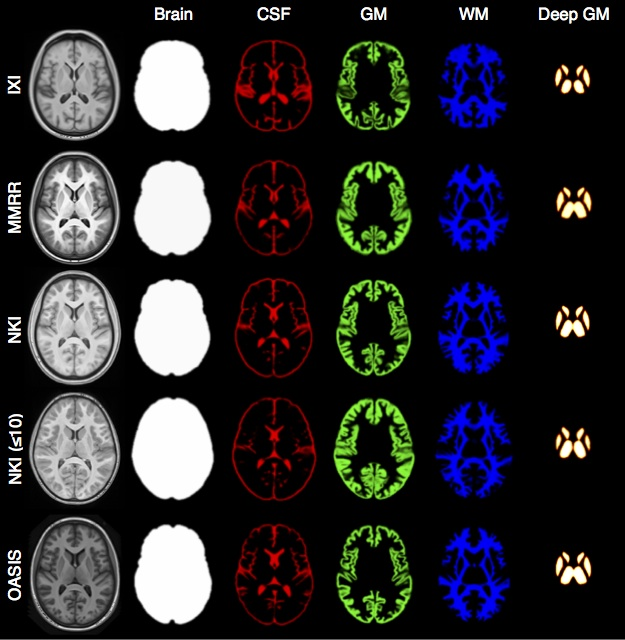
\includegraphics[width=130mm]{Figures/templateProbabilityMasks.jpg}
  \caption{\baselineskip 12pt Axial slices from each of the five T1 templates including the corresponding
  probability masks used for brain extraction and brain tissue segmentation.  Not shown
  are the prior probability maps for brain stem and cerebellum regions.
  }
  \label{fig:templateMasks}
\end{figure}


\subsection{Processing miscellany}

Given the documented variability in FreeSurfer results with version and
operating system \citep{gronenschild2012} (as we would expect with our own ANTs pipeline),
all data were processed using the same ANTs and FreeSurfer versions on the same 
hardware platform.  Processing was performed using the Linux (CentOS release 6.4) 
cluster at the University 
of Virginia%
\footnote{
http://www.uvacse.virginia.edu/
}
using single-threading with a maximal requested memory footprint of 8 gb for ANTs 
and 4 gb for FreeSurfer.  The development version of ANTs was used for processing 
(git commit tag: 69d3a5a6c7125ccf07a9e9cf6ef29f0b91e9514f, date Dec. 11, 2013).  
FreeSurfer version 5.3 x86\_64 for CentOs was downloaded 
on 5 December, 2013 (``freesurfer-Linux-centos6\_x86\_64-stable-pub-v5.3.0'', release
date: 15 May, 2013). 

We visually inspected all brain extraction and segmentation results from the ANTs and FreeSurfer pipelines. This cursory quality control step consisted of a script which displayed three cross-sectional views, one along each viewing axis in a time-series of ITK-SNAP window displays. No manual changes were made for any component of either pipeline and no change was made to the settings of either processing pipeline.

